% Taller 4 -- Punto 4: Taller de lógica difusa (adicional): modelos difusos de 4 y de 2 sensores del robot.  Compilar:  make punto4
% Las cifras (\cifra...) y las tablas salen de desarrollo/exportar_informe.py a partir del cuaderno ejecutado.
\documentclass[11pt,letterpaper]{article}
\usepackage{ud-informe}
% Acento azul: el logo del programa (MCIC) es azul, así que se usa la gama azur del manual de marca en lugar del rojo.
% Para volver al rojo institucional de la plantilla, borrar estas dos líneas.
\colorlet{udrojo}{udazul}
\definecolor{udrojoosc}{HTML}{0C6F96}
% Generado por desarrollo/exportar_informe.py: NO editar a mano.
\newcommand{\cifrapropMamdani}{5,5586}
\newcommand{\cifrapropSugeno}{5,3445}
\newcommand{\cifrapropIrisReglas}{16}
\newcommand{\cifrapropIrisAcc}{0,889}
\newcommand{\cifrapropIrisAri}{0,729}
\newcommand{\cifratodoUnoA}{flavanoids}
\newcommand{\cifratodoUnoB}{proline}
\newcommand{\cifratodoUnoC}{OD280/OD315}
\newcommand{\cifratodoUnoD}{alcohol}
\newcommand{\cifratodoUnoFA}{188}
\newcommand{\cifratodoUnoFB}{149}
\newcommand{\cifratodoUnoFC}{127}
\newcommand{\cifratodoUnoFD}{100}
\newcommand{\cifrapropCurvaReglas}{0,2: 66, 0,3: 15, 0,4: 8, 0,5: 4, 0,6: 4, 0,7: 3, 0,8: 3, 0,9: 3, 1,0: 3}
\newcommand{\cifrapropRidgeSin}{45,1\,\%}
\newcommand{\cifrapropCvTresRidge}{90,3\,\%}
\newcommand{\cifrapropTestTresRidge}{96,3\,\%}
\newcommand{\cifrapropPureza}{0,927}
\newcommand{\cifrapropAri}{0,794}
\newcommand{\cifrapropFpc}{0,690}
\newcommand{\cifrapropFrontera}{20}
\newcommand{\cifrapropPurezaKm}{0,927}
\newcommand{\cifrapropMalAgrupados}{13}
\newcommand{\cifrapropRMejor}{0,8}
\newcommand{\cifrapropReglasMejor}{3}
\newcommand{\cifrapropAccMejor}{94,4\,\%}
\newcommand{\cifrapropCvUno}{45,1\,\%}
\newcommand{\cifrapropCvDos}{95,2\,\%}
\newcommand{\cifrapropCvTres}{96,0\,\%}
\newcommand{\cifratuneEntAntes}{0,145}
\newcommand{\cifratuneEntDesp}{0,095}
\newcommand{\cifratuneValAntes}{0,260}
\newcommand{\cifratuneValDesp}{0,254}
\newcommand{\cifratuneEntSin}{0,0006}
\newcommand{\cifratuneValSin}{0,384}
\newcommand{\cifratuneIter}{1}
\newcommand{\cifratuneIters}{40}
\newcommand{\cifratuneAccAntes}{90,7\,\%}
\newcommand{\cifratuneAccDesp}{94,4\,\%}
\newcommand{\cifratuneValSubida}{47}
\newcommand{\cifraveinteWMdos}{0,806 $\pm$ 0,049}
\newcommand{\cifraveinteReglasWMdos}{9,7 $\pm$ 1,2}
\newcommand{\cifraveinteWMtres}{0,865 $\pm$ 0,047}
\newcommand{\cifraveinteReglasWMtres}{24,1 $\pm$ 3,4}
\newcommand{\cifraveinteWMcuatro}{0,931 $\pm$ 0,036}
\newcommand{\cifraveinteReglasWMcuatro}{41,9 $\pm$ 2,9}
\newcommand{\cifraveinteSubTres}{0,881 $\pm$ 0,078}
\newcommand{\cifraveinteReglasSubTres}{14,8 $\pm$ 2,8}
\newcommand{\cifraveinteSubCinco}{0,956 $\pm$ 0,024}
\newcommand{\cifraveinteReglasSubCinco}{5,0 $\pm$ 0,9}
\newcommand{\cifraveinteSubOcho}{0,946 $\pm$ 0,024}
\newcommand{\cifraveinteReglasSubOcho}{3,0 $\pm$ 0,0}
\newcommand{\cifraveinteArbol}{0,894 $\pm$ 0,044}
\newcommand{\cifrapropSelDistintas}{2}
\newcommand{\cifrapropPermMax}{95,6\,\%}
\newcommand{\cifrapropPermMin}{90,4\,\%}
\newcommand{\cifrapropPermWM}{86,5\,\%}
\newcommand{\cifraadicN}{5456}
\newcommand{\cifraadicTrain}{3856}
\newcommand{\cifraadicTest}{1600}
\newcommand{\cifraadicDupCuatro}{50}
\newcommand{\cifraadicDupDos}{279}
\newcommand{\cifraadicRacha}{6,5}
\newcommand{\cifraadicCambios}{395}
\newcommand{\cifraadicSharp}{2097}
\newcommand{\cifraadicSlightR}{826}
\newcommand{\cifraadicForward}{2205}
\newcommand{\cifraadicSlightL}{328}
\newcommand{\cifraadicDosReglas}{6}
\newcommand{\cifraadicDosW}{0,02}
\newcommand{\cifraadicDosAcc}{99,81}
\newcommand{\cifraadicDosBal}{99,88}
\newcommand{\cifraadicDosF}{99,88}
\newcommand{\cifraadicDosMF}{2\,$\times$\,3}
\newcommand{\cifraadicCuatroReglas}{24}
\newcommand{\cifraadicCuatroW}{0,02}
\newcommand{\cifraadicCuatroAcc}{99,50}
\newcommand{\cifraadicCuatroBal}{99,39}
\newcommand{\cifraadicCuatroF}{99,45}
\newcommand{\cifraadicCuatroMF}{2\,$\times$\,3\,$\times$\,2\,$\times$\,2}
\newcommand{\cifraadicCorteFrente}{0,9005}
\newcommand{\cifraadicCorteIzqA}{0,4945}
\newcommand{\cifraadicCorteIzqB}{0,9015}
\newcommand{\cifraadicAutoDosMin}{91,4\,\%}
\newcommand{\cifraadicAutoDosMax}{96,1\,\%}
\newcommand{\cifraadicAutoCuatroMin}{78,7\,\%}
\newcommand{\cifraadicAutoCuatroMax}{95,2\,\%}
\newcommand{\cifraadicAutoReglasMin}{48}
\newcommand{\cifraadicAutoReglasMax}{100}
\newcommand{\cifraadicKnnBloques}{85,6\,\%}
\newcommand{\cifraadicKnnMuestra}{94,0\,\%}
\newcommand{\cifraadicKnnInfla}{8,3}
\newcommand{\cifraadicMamdaniDosCero}{97,8\,\%}
\newcommand{\cifraadicMamdaniDosGrande}{58,2\,\%}
\newcommand{\cifraadicGanadoraDosGrande}{92,6\,\%}


\renewcommand{\UDtitulo}{Lógica difusa para el movimiento de un robot}
\renewcommand{\UDsubtitulo}{Modelos de 4 y de 2 sensores a partir del análisis de datos}
\renewcommand{\UDtipo}{Taller 4 -- Punto 4 -- Informe de ejecución}
\renewcommand{\UDasignatura}{Inteligencia Computacional Aplicada}
\renewcommand{\UDdocente}{Cesar Andrey Perdomo Charry}
\renewcommand{\UDestudiantes}{Juan Felipe Rodríguez Galindo -- 20261595004}
\renewcommand{\UDencabezado}{Taller 4 -- Punto 4: modelos difusos del robot}
\newcommand{\pts}{\,pts}

\begin{document}
\UDportada

%% ---------------------------------------------------------------------------------------------
\section{Enunciado y datos}

A partir del análisis de datos se piden \textbf{dos modelos de lógica difusa} para clasificar el movimiento de un robot, uno con 4 sensores de entrada y otro con 2. Las funciones de pertenencia (MF) de cada variable se deben
definir con histogramas, histogramas con clase y nube de puntos; el número de reglas es el producto de las MF por variable, con un \textbf{máximo de 100}.

Los datos son \cifraadicN{} lecturas de un robot que sigue una pared (los archivos no traen encabezado; los nombres \textit{frente}, \textit{izquierda}, \textit{derecha} y \textit{atrás} se toman del conjunto original de la UCI,
y el análisis es coherente con esa lectura). La salida son cuatro movimientos, ordenados de giro cerrado a la derecha a giro leve a la izquierda: \textit{Sharp-Right-Turn} (\cifraadicSharp), \textit{Slight-Right-Turn} (\cifraadicSlightR),
\textit{Move-Forward} (\cifraadicForward) y \textit{Slight-Left-Turn} (\cifraadicSlightL). Hay \cifraadicDupCuatro{} filas duplicadas (\cifraadicDupDos{} en el archivo de 2 sensores) y lecturas saturadas en 5,0.

\textbf{Son una serie en el tiempo:} hay solo \cifraadicCambios{} cambios de clase y una racha típica dura \cifraadicRacha{} lecturas, es decir, las lecturas vecinas son casi idénticas. Por eso la prueba se forma con \textbf{bloques completos de 100 lecturas consecutivas}
(30\,\% de los bloques: \cifraadicTrain{} lecturas de entrenamiento y \cifraadicTest{} de prueba) y no con lecturas sueltas.

\begin{figure}[H]
\centering
\begin{tikzpicture}[node distance=0.4cm]
  \node[caja] (a) {Sensores\\\footnotesize 4 o 2 distancias};
  \node[caja, right=of a] (b) {Fuzzificación\\\footnotesize grados $\mu$ por MF};
  \node[hecho, right=of b] (c) {Base de reglas\\\footnotesize una por combinación};
  \node[caja, right=of c] (d) {Inferencia\\\footnotesize $Y$ = producto};
  \node[caja, right=of d] (e) {Decisión\\\footnotesize regla ganadora};
  \draw[flecha] (a) -- (b); \draw[flecha] (b) -- (c); \draw[flecha] (c) -- (d); \draw[flecha] (d) -- (e);
\end{tikzpicture}
\caption{Esquema del sistema difuso construido (para 4 y para 2 sensores).}
\end{figure}

%% ---------------------------------------------------------------------------------------------
\section{Análisis de datos}

\textbf{Histogramas con clase (figura~\ref{fig:hist}).} En \textit{frente}, \textit{Sharp-Right-Turn} ocupa todo el pico de la izquierda y termina de forma abrupta en 0,9; a la derecha de ese valor no aparece. En \textit{izquierda},
\textit{Slight-Right-Turn} se acumula por debajo de 0,5, \textit{Move-Forward} ocupa de 0,5 a 0,9 y \textit{Slight-Left-Turn} queda aislado en valores altos. En \textit{derecha} y \textit{atrás} las cuatro curvas se superponen: no hay un valor donde cambie la clase.

\begin{figure}[H]
\centering
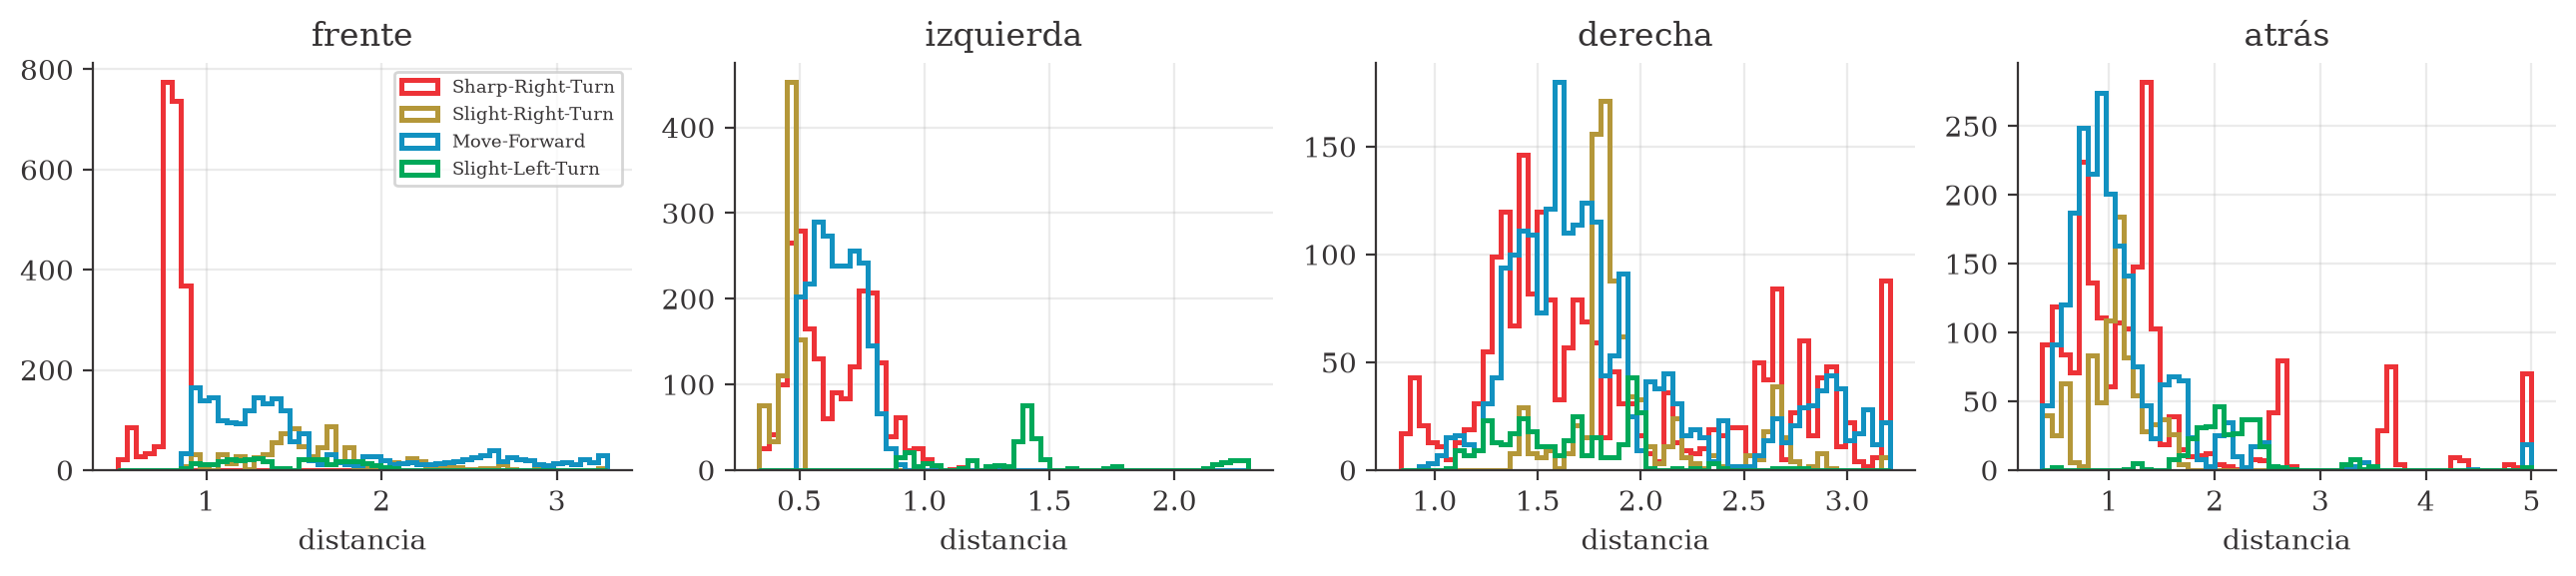
\includegraphics[width=\linewidth]{figuras/adic_f03_histogramas_clase.png}
\caption{Histograma con clase de cada sensor.}\label{fig:hist}
\end{figure}

\textbf{Nube de puntos (figura~\ref{fig:nube}).} El histograma marginal de \textit{izquierda} engaña: \textit{Sharp-Right-Turn} se reparte por todos sus valores y tapa el corte de 0,9. Solo en el histograma \textbf{condicionado a frente $>0{,}9$} (derecha de la figura) se ven tres bloques separados,
y la nube \textit{frente} contra \textit{izquierda} muestra que las clases forman \textbf{regiones rectangulares}: la frontera depende de una variable a la vez, son umbrales.

\begin{figure}[H]
\centering
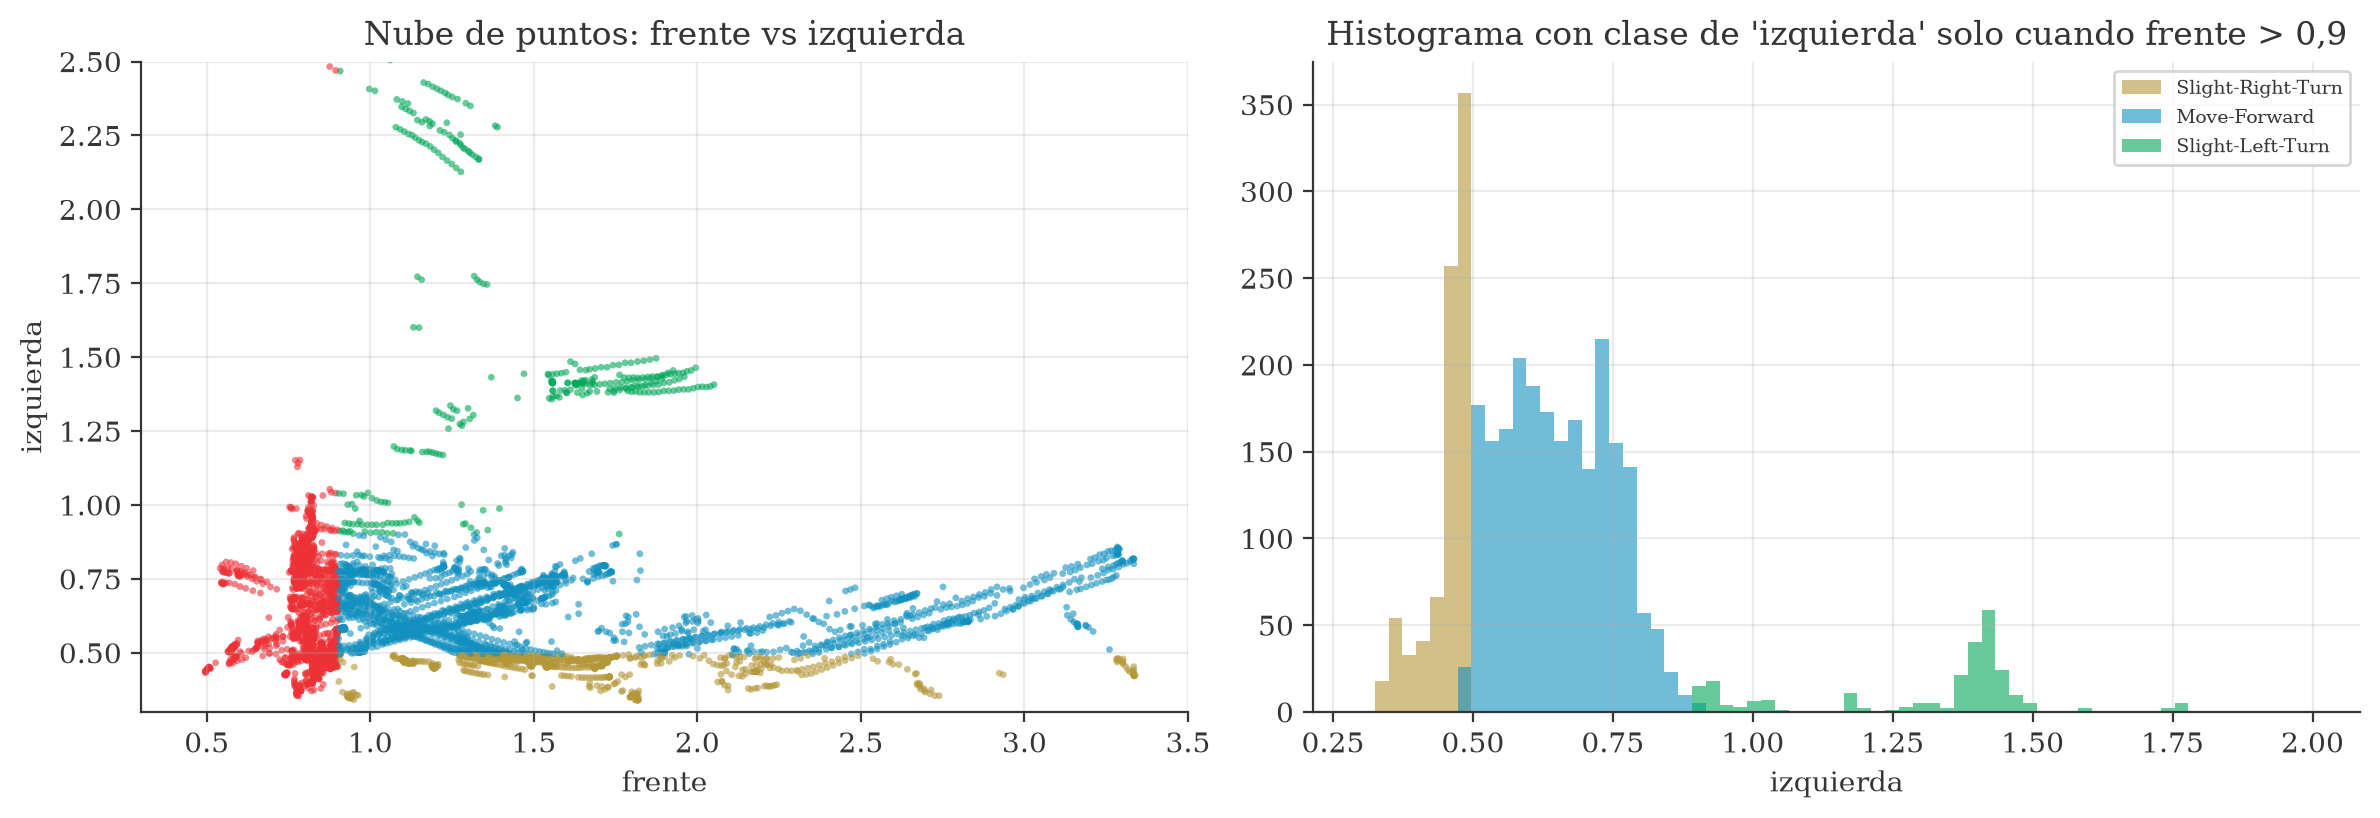
\includegraphics[width=\linewidth]{figuras/adic_f05_frente_izquierda.png}
\caption{Nube de puntos \textit{frente} contra \textit{izquierda} e histograma con clase de \textit{izquierda} condicionado a \textit{frente} $>0{,}9$.}\label{fig:nube}
\end{figure}

\begin{table}[H]
\centering\small
\caption{Relevancia de cada sensor (solo con entrenamiento).}
\begin{tabular}{lrrr}
\toprule
Sensor & F de ANOVA & Información mutua & Importancia en árbol \\
\midrule
frente & 774 & 0,793 & 0,556 \\
izquierda & 2715 & 0,577 & 0,444 \\
derecha & 9 & 0,310 & 0,000 \\
atrás & 119 & 0,329 & 0,000 \\
\bottomrule
\end{tabular}

\end{table}

Un árbol pequeño solo usa \textbf{frente} (corte \cifraadicCorteFrente) e \textbf{izquierda} (cortes \cifraadicCorteIzqA{} y \cifraadicCorteIzqB) y deja \textit{derecha} y \textit{atrás} con importancia 0. La información mutua de esos dos no es cero porque cada uno, solo, tiene alguna relación con la clase, pero es
redundante: \textbf{4 reglas nítidas con solo frente e izquierda clasifican el 100\,\% de la prueba}. Las clases parecen provenir de un controlador por umbrales: \textit{frente} $\le0{,}9$ $\to$ giro cerrado; si no, \textit{izquierda} $\le0{,}49$ $\to$ giro leve a la derecha, $\le0{,}9$ $\to$ avanzar y $>0{,}9$ $\to$ giro leve a la izquierda.

%% ---------------------------------------------------------------------------------------------
\section{Diseño de los modelos}

Los cruces de las MF (donde dos etiquetas valen 0,5) se colocan en los cortes del análisis y cada MF es un \textbf{trapecio con meseta}: vale 1 en su zona y baja a 0 en una franja de ancho $2w$ alrededor de cada corte.
El parámetro $w$ es el grado de difusividad: con $w=0$ el sistema es nítido. La base de reglas es \textbf{completa} (una por combinación) y la clase de cada una sale de los datos de entrenamiento, ponderando las clases para que la rara no se pierda; el peso de la regla es su pureza.

\begin{table}[H]
\centering\small
\caption{Funciones de pertenencia por variable y número de reglas.}
\begin{tabularx}{\linewidth}{@{}l c L L@{}}
\toprule
Variable & MF & Etiquetas & Puntos de cruce \\
\midrule
frente & 2 & cerca, lejos & \cifraadicCorteFrente \\
izquierda & 3 & muy cerca, cerca, lejos & \cifraadicCorteIzqA{} y \cifraadicCorteIzqB \\
derecha (solo en el modelo de 4) & 2 & cerca, lejos & mediana \\
atrás (solo en el modelo de 4) & 2 & cerca, lejos & mediana \\
\midrule
\multicolumn{4}{@{}l}{Reglas: \textbf{2 sensores $=2\times3=\cifraadicDosReglas$}; \textbf{4 sensores $=2\times3\times2\times2=\cifraadicCuatroReglas$} (máximo permitido: 100).} \\
\bottomrule
\end{tabularx}
\end{table}

La difusividad $w$ se eligió por validación cruzada por bloques solo con el entrenamiento: la mayor $w$ que pierde como máximo 0,2 puntos de exactitud balanceada frente al mejor valor, que resultó $w=\cifraadicDosW$ para ambos modelos (una franja de 0,04 alrededor de cada corte).
Derecha y atrás llevan 2 MF cada una (cruce en la mediana) solo para cumplir con tener las 4 entradas; el análisis indica que podrían omitirse.

\begin{figure}[H]
\centering
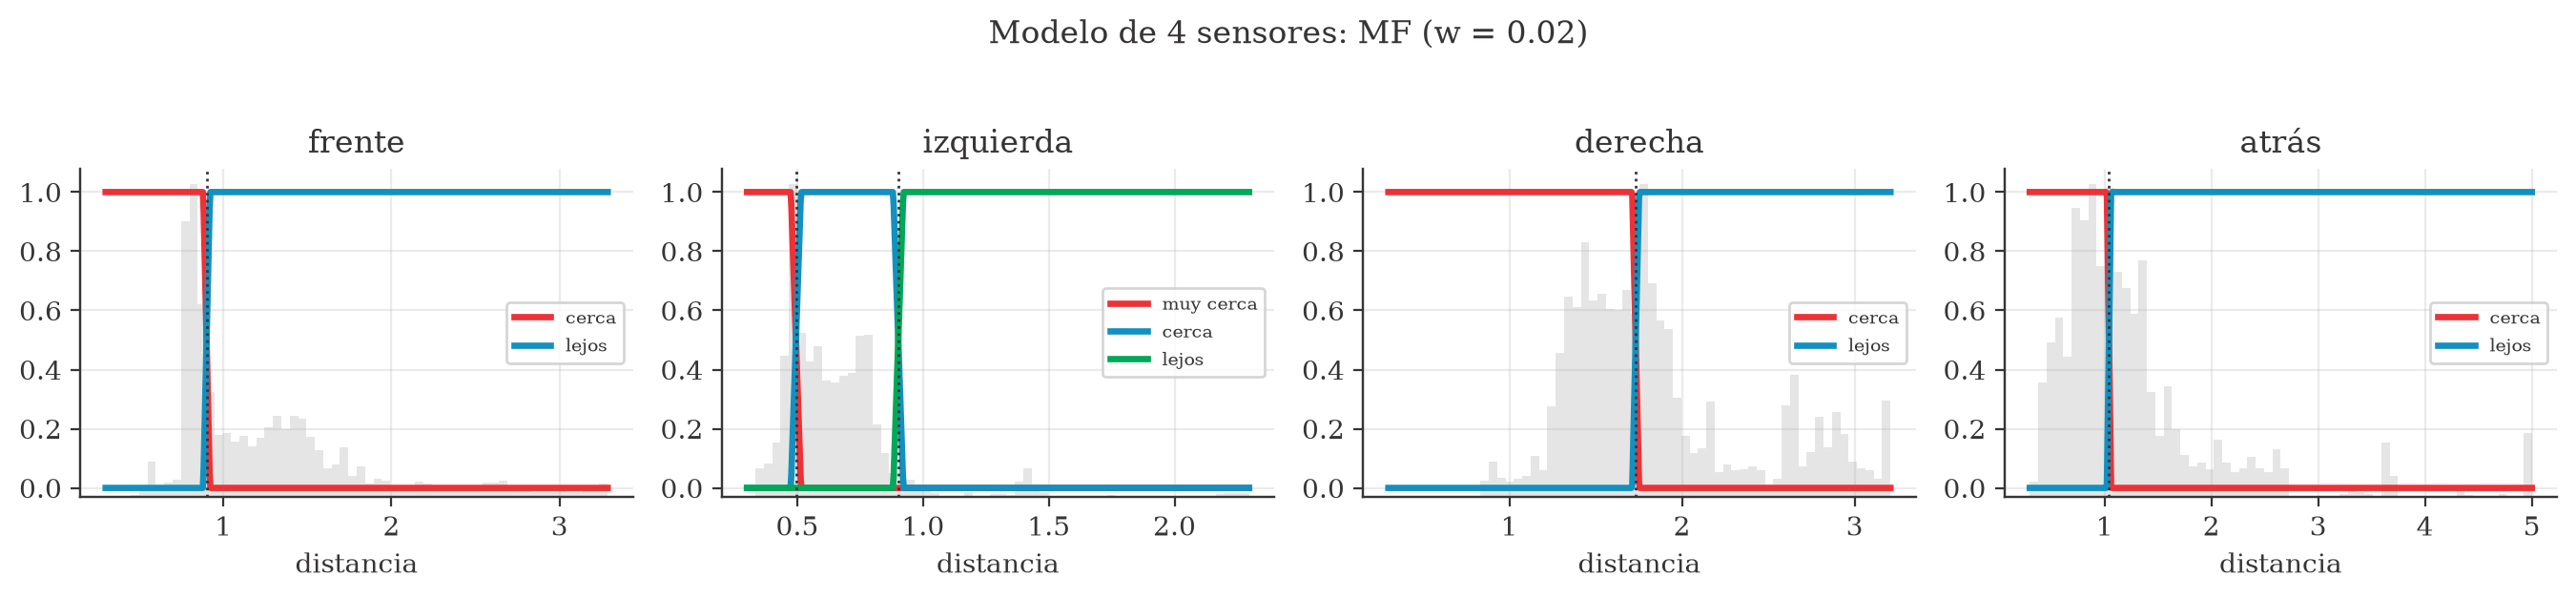
\includegraphics[width=\linewidth]{figuras/adic_f07_mf_4sensores.png}
\caption{Funciones de pertenencia del modelo de 4 sensores sobre el histograma de cada variable (el de 2 sensores usa las dos primeras).}
\end{figure}

\begin{table}[H]
\centering\small
\caption{Las 6 reglas del modelo de 2 sensores.}
\begin{tabular}{llll}
\toprule
Si frente es & y izquierda es & Entonces & Peso \\
\midrule
cerca & muy cerca & Sharp-\allowbreak Right-\allowbreak Turn & 0,98 \\
cerca & cerca & Sharp-\allowbreak Right-\allowbreak Turn & 0,99 \\
cerca & lejos & Sharp-\allowbreak Right-\allowbreak Turn & 0,94 \\
lejos & muy cerca & Slight-\allowbreak Right-\allowbreak Turn & 0,97 \\
lejos & cerca & Move-\allowbreak Forward & 0,90 \\
lejos & lejos & Slight-\allowbreak Left-\allowbreak Turn & 1,00 \\
\bottomrule
\end{tabular}

\end{table}

\begin{figure}[H]
\centering
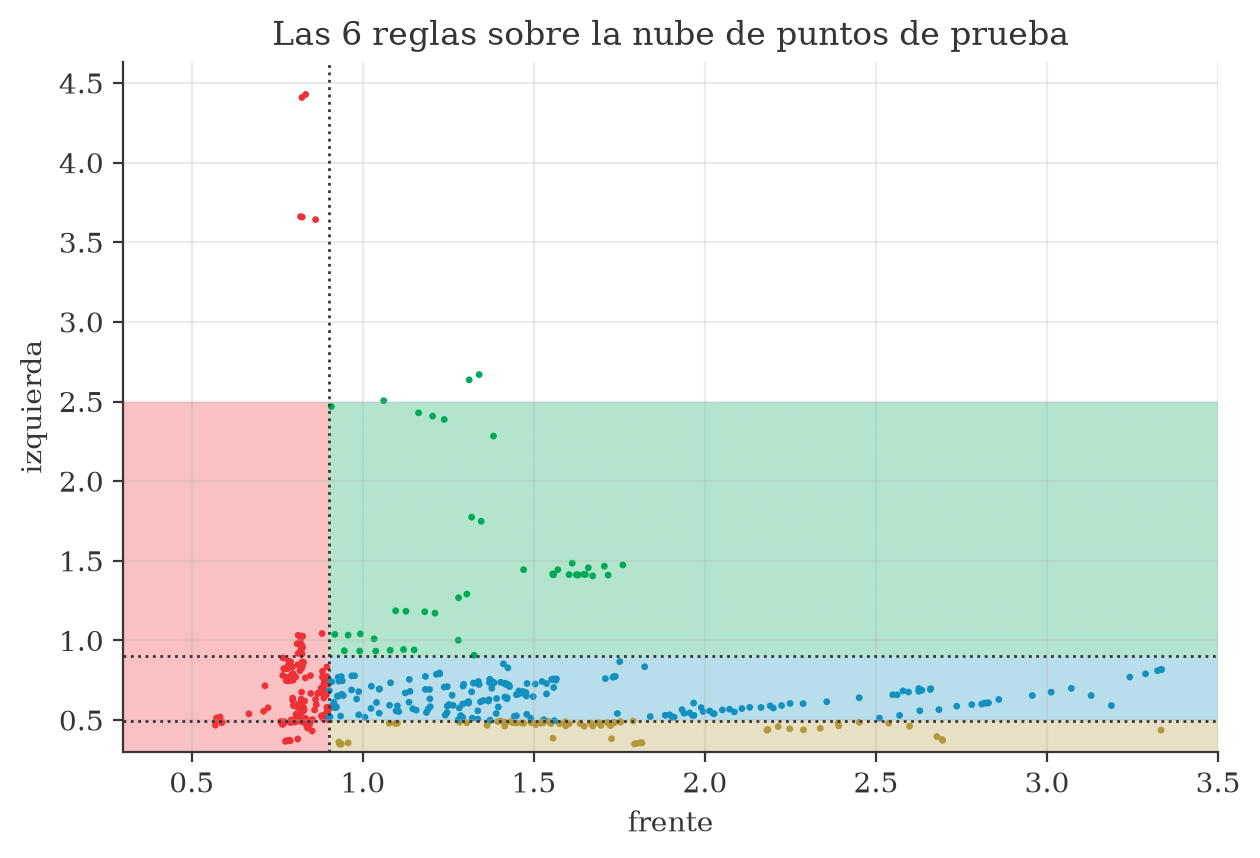
\includegraphics[width=0.5\linewidth]{figuras/adic_f08_mapa_reglas.png}
\caption{Región que gana cada regla en el plano \textit{frente}--\textit{izquierda}, sobre la nube de puntos de prueba.}
\end{figure}

%% ---------------------------------------------------------------------------------------------
\section{Resultados}

\begin{table}[H]
\centering\small
\caption{Resultados en los bloques de prueba (\cifraadicTest{} lecturas).}
\begin{tabular}{lrrrrrr}
\toprule
Modelo & MF por variable & Reglas & $w$ & Exactitud & Exact. balanceada & F1 macro \\
\midrule
2 sensores & 2 $\times$ 3 & 6 & 0,02 & 99,81\,\% & 99,88\,\% & 99,88\,\% \\
4 sensores & 2 $\times$ 3 $\times$ 2 $\times$ 2 & 24 & 0,02 & 99,50\,\% & 99,39\,\% & 99,45\,\% \\
\bottomrule
\end{tabular}

\end{table}

El modelo de \textbf{2 sensores} (6 reglas) acierta \cifraadicDosAcc\,\% y el de \textbf{4 sensores} (24 reglas) \cifraadicCuatroAcc\,\%. Los errores están a menos de 0,002 de un corte en la variable que decide (por ejemplo, \textit{frente} $=0{,}901$ cuando el corte es $0{,}9005$),
justo donde las dos etiquetas valen casi lo mismo. El modelo de 4 sensores es ligeramente peor porque sus dos variables extra no aportan información y solo multiplican las reglas por 4.

\textbf{El análisis importa.} Con el mismo límite de 100 reglas, los diseños automáticos (uniformes, por cuantiles o por Fuzzy C-Means, con el número de MF elegido por validación cruzada) logran de \cifraadicAutoDosMin{} a \cifraadicAutoDosMax{} con 2 sensores y de \cifraadicAutoCuatroMin{} a \cifraadicAutoCuatroMax{} con 4, usando de \cifraadicAutoReglasMin{} a \cifraadicAutoReglasMax{} reglas.

\begin{table}[H]
\centering\small
\caption{Diseños de MF con el límite de 100 reglas (CV = exactitud balanceada en validación cruzada por bloques).}
\begin{tabular}{llrrrrr}
\toprule
Modelo & Diseño de las MF & MF & Reglas & CV & Exactitud & Exact. bal. \\
\midrule
2 sensores & uniforme (auto.) & 6-10 & 60 & 95,4\,\% & 91,4\,\% & 94,2\,\% \\
2 sensores & cuantiles (auto.) & 6-8 & 48 & 96,7\,\% & 94,4\,\% & 96,3\,\% \\
2 sensores & fcm (auto.) & 8-10 & 80 & 95,6\,\% & 96,1\,\% & 97,3\,\% \\
2 sensores & cortes del análisis & 2-3 & 6 & 99,8\,\% & 99,8\,\% & 99,9\,\% \\
4 sensores & uniforme (auto.) & 5-5-2-2 & 100 & 86,7\,\% & 78,7\,\% & 80,8\,\% \\
4 sensores & cuantiles (auto.) & 3-4-3-2 & 72 & 95,4\,\% & 95,2\,\% & 96,3\,\% \\
4 sensores & fcm (auto.) & 5-5-2-2 & 100 & 90,0\,\% & 83,6\,\% & 83,0\,\% \\
4 sensores & cortes del análisis & 2-3-2-2 & 24 & 99,8\,\% & 99,5\,\% & 99,4\,\% \\
\bottomrule
\end{tabular}

\end{table}


\textbf{Cuidado con la partición.} Con lecturas sueltas en lugar de bloques, kNN pasa de \cifraadicKnnBloques{} a \cifraadicKnnMuestra{} en el modelo de 4 sensores (\textbf{+\cifraadicKnnInfla\pts} de fuga entre lecturas vecinas); los modelos con cortes del análisis casi no cambian porque no memorizan: aprenden umbrales.

\begin{table}[H]
\centering\small
\caption{Exactitud en prueba con partición por bloques frente a partición muestra a muestra.}
\begin{tabular}{llrrr}
\toprule
Modelo & Método & Por bloques & Muestra a muestra & Diferencia \\
\midrule
2 sensores & difuso con cortes del análisis & 99,8\,\% & 99,8\,\% & 0,01\,pts \\
2 sensores & difuso cuantiles & 94,4\,\% & 96,5\,\% & 2,08\,pts \\
2 sensores & kNN (k = 15) & 95,0\,\% & 97,0\,\% & 1,95\,pts \\
2 sensores & árbol (60 hojas) & 100,0\,\% & 100,0\,\% & 0,00\,pts \\
4 sensores & difuso con cortes del análisis & 99,5\,\% & 99,6\,\% & 0,13\,pts \\
4 sensores & difuso cuantiles & 95,2\,\% & 94,0\,\% & $-$1,30\,pts \\
4 sensores & kNN (k = 15) & 85,6\,\% & 94,0\,\% & 8,33\,pts \\
4 sensores & árbol (60 hojas) & 100,0\,\% & 100,0\,\% & 0,00\,pts \\
\bottomrule
\end{tabular}

\end{table}

%% ---------------------------------------------------------------------------------------------
\section{Difusividad y variante Mamdani}

Con \textbf{regla ganadora} la exactitud cae poco y de forma gradual al aumentar $w$ (\cifraadicGanadoraDosGrande{} con $w=0{,}2$, 2 sensores). Con \textbf{Mamdani y centroide} (las clases ordenadas de giro cerrado a la derecha a giro leve a la izquierda, salida redondeada) la caída es mucho más rápida:
\cifraadicMamdaniDosCero{} con $w=0{,}005$ y \cifraadicMamdaniDosGrande{} con $w=0{,}2$. Las clases son categorías y el centroide mezcla reglas vecinas en un número intermedio que, al redondear, puede caer en una tercera clase. Para \textbf{clasificar} conviene la regla ganadora;
la salida Mamdani tiene sentido como señal de dirección continua. Nuestro Mamdani coincide con \texttt{scikit-fuzzy} (diferencia menor de 0,02 en 150 puntos).

\begin{table}[H]
\centering\small
\caption{Exactitud en prueba según la difusividad $w$ y la forma de producir la salida.}
\begin{tabular}{lrrrr}
\toprule
$w$ & 2 sens. ganadora & 2 sens. Mamdani & 4 sens. ganadora & 4 sens. Mamdani \\
\midrule
0,000 & 100,0\,\% & 100,0\,\% & 100,0\,\% & 100,0\,\% \\
0,005 & 100,0\,\% & 97,8\,\% & 99,9\,\% & 97,8\,\% \\
0,010 & 100,0\,\% & 95,9\,\% & 99,8\,\% & 95,9\,\% \\
0,020 & 99,8\,\% & 94,5\,\% & 99,5\,\% & 94,2\,\% \\
0,050 & 98,8\,\% & 89,2\,\% & 98,2\,\% & 89,0\,\% \\
0,100 & 96,8\,\% & 81,9\,\% & 96,0\,\% & 82,1\,\% \\
0,200 & 92,6\,\% & 58,2\,\% & 91,0\,\% & 57,9\,\% \\
\bottomrule
\end{tabular}

\end{table}

%% ---------------------------------------------------------------------------------------------
\section{Conclusiones y límites}
\begin{enumerate}
  \item El análisis de datos define las MF: las clases separan por \textbf{umbrales sobre dos sensores} (frente en 0,9; izquierda en 0,49 y 0,9); derecha y atrás no aportan.
  \item \textbf{2 sensores:} $2\times3=\cifraadicDosReglas$ reglas, \cifraadicDosAcc\,\% de exactitud y \cifraadicDosBal\,\% de exactitud balanceada. \textbf{4 sensores:} $2\times3\times2\times2=\cifraadicCuatroReglas$ reglas, \cifraadicCuatroAcc\,\% y \cifraadicCuatroBal\,\%. Ambos respetan el máximo de 100.
  \item Más reglas no es mejor: los diseños automáticos con hasta 100 reglas rinden de \cifraadicAutoCuatroMin{} a \cifraadicAutoDosMax; con series de tiempo, la partición muestra a muestra infla los resultados.
  \item \textbf{Límites:} nombres de sensores tomados del conjunto original; la regla parece de un controlador por umbrales, así que no se extrapola a otro robot sin repetir el análisis; una sola partición por bloques (semilla 42).
\end{enumerate}

\textbf{Reproducir:} \texttt{make notebooks} (menos de 2 minutos); semilla 42; 19 verificaciones \texttt{[OK]}. Reglas en \texttt{resultados/reglas\_2\_sensores.csv} y \texttt{reglas\_4\_sensores.csv}.

\end{document}
